\documentclass[a4paper,11pt,phdthesis,singlespace,twoside]{cssethesis}

\usepackage{harvard} % Use the Harvard bibliography and citation package
\usepackage{graphicx}
\usepackage{epstopdf}
\usepackage{mathptmx}
\usepackage{times}

\usepackage{algorithm}
\usepackage{enumitem}

\usepackage{listings}
\usepackage{color}
\usepackage{apacite}


\thesisauthor{Viet Vo}
\thesisauthorpreviousdegrees{BSc., MSc.} % Optional
\thesisdepartment{Caulfield School of Information Technology}
\thesisauthorstudentid{26356988} % Needed for litreview
\thesisauthoremail{viet.vo\@@monash.edu} 

%\thesismonth{October} % Optional. Current month is used if this is not set
%\thesisyear{2015} % Optional. Current year is used if this is not set
\thesistitle{The Effects of Group Member's Parameters on Human Crowd Modelling}
\thesissupervisor{Prof. Bernd Meyer}
\thesissupervisoremail{bernd.meyer\@@monash.edu} 
\thesisassocsupervisor{Dr. Aldeida Aleti} 
\thesisassocsupervisoremail{aldeida.aleti\@@monash.edu} 

% start the document
\begin{document}

\frontmatter					% start the thesis front matter.

\thesistitlepage				% Generate the title page.
%\thesiscopyrightpage			% Generate the copyright page.
%\thesisdedicationpage			% Generate a dedication page (optional)
\tableofcontents				% Generate a table of contents.
\listoftables					% Generate a list of tables (optional).
\listoffigures					% Generate a list of figures (optional).

\begin{thesisabstract}			% generate the abstract page.
This thesis introduces
\end{thesisabstract}                 

\thesisdeclarationpage			% generate the declaration page (optional).

%\begin{thesisacknowledgments}	% generate the acknowledgements page (optional).
%I would like to thank everyone who helped to make this possible. It has
%been an incredible journey of self-discovery, and I love every last one of
%you\ldots
%\end{thesisacknowledgments}   

%%%%%%%%%%%%%%%%%%%%%%%%%%%%%%%%%%%%%%%%%%%%%%%%%%%%%%%%%%%%%%%%%%%%%%%%%%%%%%
%%
%% Main matter 
%%
\mainmatter						% start the thesis body.

\chapter{Introduction}
Since over 70\% of the world population is predicted to live in cities by 2050 \cite{Weidmann2012}, rapid urbanization and population growth will be inevitable challenges in the effort of planning infrastructure, estimating traffic needs and capacities, and increasing the safety of pedestrians. With the increase in the number of public events and the number of accidents during these events since the crush disaster happened at the Station Nightclub, USA (2003) \cite{Evers2011}, the demand for realistic crowd simulation models becomes important for risk management in urban design and crowd safety. To develop realistic simulation models, various studies have been conducted in order to understand and simulate behaviours which can emerge in both normal and emergency situations such as groups of pedestrians moving with or competing against each other.

Group cohesion behaviour is the behaviour of objects moving towards the average positions of their neighbors over the time \cite{Reynolds1987}. The definition of this behaviour was motivated by the visual observation of coherently flying objects. The behaviour has been investigated widely on the collective motion of different flocking organisms including homing pigeon flocks \cite{Kattas2012}, fish schools \cite{Miller2013}, and bacteria colony \cite{Cisneros2007}. 

Human group cohesion behaviour is observed by its cohesion degree and formation. Cohesion degree denotes the average distance to the group’s centre of mass from each group member while observable human group formations are V-like, line-abreast, U-like, or river-like \cite {Helbing2005}. Group cohesion behaviour is important in both normal and evacuation scenarios. In normal situations, group cohesion behaviour can affect the speed and movement direction of pedestrians who are not belonging to any group. In human behaviour research, the frequency of group cohesion behaviour’s occurrence has been observed at different places in the UK with the percentages of 37\% at train station, 50\% at shopping centre, 28\% at university campus, 50\%, at Clumber Street \cite{Singh2009}. Pedestrians in the same group might be family members, colleagues. In crowd disasters, pedestrians evacuate with group rather than escape individually. Groups of families and friends with strong ties, stay together and evacuate together have been emphasized through socio-psychological research area \cite {Mawson2005}. They may move irrationally to maintain its cohesion and consequently become obstacles for other pedestrians \cite{Aguirre2011}.

\chapter{Literature Review}

In this chapter I will demonstrate some of the extended citation
capabilities provided by the {\sf natbib} package \cite{Dal1999}. It
replaces the standard \LaTeX\ \verb+\cite+ command with two basic forms of
citation command: \verb+\citep+ and \verb+\citet+, as well as providing
several other very useful ones.

The \verb+\citep+ command is best used when placing a citation at the end
of sentence or phrase (as above).  In the {\sf natbib} documentation, this
is referred to as a \emph{parenthetical citation}.%
\footnote{For ease of conversion from exisiting \LaTeX\ documents, you
might find it useful to place
\texttt{$\backslash$renewcommand\{$\backslash$cite\}\{$\backslash$citep\}}
in the preamble of the document, since any existing standard
\texttt{$\backslash$cite} commands should almost certainly be treated as
\texttt{$\backslash$citep}.}

When you want to refer to the authors of a particular work, typically at
the start of a sentence, a parenthetical citation is not appropriate. This
is particularly so if you are using a numerical or symbolic citation style.
You should \emph{not} start a sentence with
\begin{quote}
[2] says that this is most certainly \ldots
\end{quote}
In such situations you really need to give the authors' names. The
\verb+\citet+ command produces \emph{textual citations}, which allows you
to produce things like:
\begin{quote}
\citet{Ade1983} describes a means by which textures may be
characterized \ldots another approach is given in \citet{DeV1998}.

\citet{AGR1996} note that humans have little or no difficulty in
perceiving shape, yet find it extremely difficult to \emph{describe} what
they perceive.
\end{quote}

Note that an abbreviated version of the authors' names has been produced in
the third example above.  It is often desirable to have the full list of
authors' names given when a work  is first cited, and an abbreviated list
thereafter. This can be achieved by passing the \texttt{longnamesfirst}
option to {\sf natbib} when the package is used. This will produce
an initial citation like:
\begin{quote}
\citet*{AGR1996} note that humans have little or no difficulty in
perceiving shape, yet find it extremely difficult to \emph{describe} what
they perceive.
\end{quote}

Both the \verb+\citep+ and \verb+\citet+ can take two optional arguments.
If just one is provided,  its text will appear as a ``post-note'' after the
citation details. If two arguments are provided, the first defines a
pre-note, and the second a post-note. Here is an example:
\begin{quote}
\verb+\citep[Ch.~3]{AaK1989}+ \ldots{} \citep[Ch.~3]{AaK1989}\\
\verb+\citep[see][Ch.~3]{AaK1989}+ \ldots{} \citep[see][Ch.~3]{AaK1989}\\
\end{quote}

These examples only scratch the surface of what the {\sf natbib} package
can do. To discover the full power of the package, see the documentation at
CTAN \citep{Dal1999}. You probably already have it on your system. Try
\verb+locate natbib.dvi+ at the command line.
 % this causes a page-break, so put the \chapter command in
				 % the file to be included - I don't know why this happens :(

\chapter{Figures and Tables}
Here we will test that references to figures and tables work correctly.

\section{Figures}
\begin{figure}[ht]
\begin{center}
\resizebox{100mm}{!}{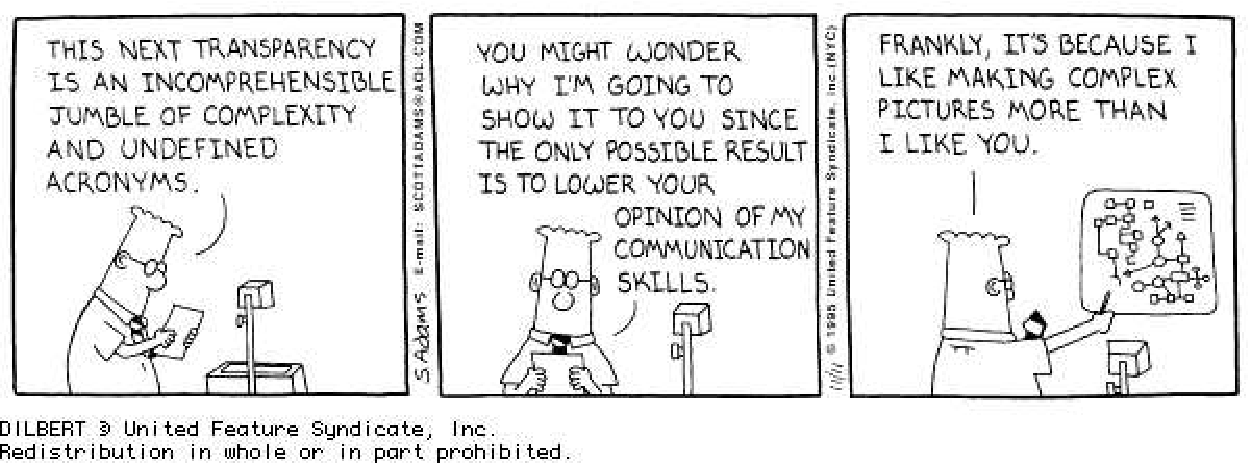
\includegraphics{dilbert_complexpictures}}
\end{center}
\caption{An example of a figure.}
\label{fig:example}
\end{figure}
See Figure~\ref{fig:example}.

\section{Tables}
\begin{table}
\begin{center}
\begin{tabular}{lcr}
23121 & 1212 & 232 \\ \hline  
cat & frog & dog
\end{tabular}
\end{center}
\caption{An example of a table}
\label{tab:example}
\end{table}
See Table~\ref{tab:example}.

\subsection{Referencing test}
See Table~\ref{tab:example} and Figure~\ref{fig:example}.

% another chapter
\chapter{Method}
Lorem ipsum dolor sit amet, consetetur sadipscing elitr,  sed diam nonumy
eirmod tempor invidunt ut labore et dolore magna aliquyam erat, sed diam
voluptua. 

\appendix % all \chapter{..} commands after this will generate appendices

\chapter{This appendix should get a letter}
\label{app:example}
An appendix before the backmatter gets an automatically generated letter by
which it can be referred to. This is Appendix~\ref{app:example}.

\chapter{Simulation Source Code}
You may want to investigate the \texttt{lgrind} program and package if you
wish to include source code in your thesis

%%%%%%%%%%%%%%%%%%%%%%%%%%%%%%%%%%%%%%%%%%%%%%%%%%%%%%%%%%%%%%%%%%%%%%%%%%%%%%
%%
%% Back matter 
%%

\backmatter						% start the thesis back matter
\bibliographystyle{apacite}
\bibliography{confirmationmonashbib}

\chapter{Last Thing} 
This sort of appendix has no letter. 


\end{document}
